\documentclass[aspectratio=169]{beamer}              % only frames

% for themes, etc.
\mode<presentation>
\usetheme{Madrid} 
\usecolortheme{crane}

%\usepackage{times}  % fonts are up to you
% The usual suspects
\usepackage{multirow, booktabs, dcolumn, color, graphicx} % Tables\usepackage{graphicx}
\usepackage{amsmath,amssymb,amsthm}
% Strikethrough text
\usepackage{soul}
% Adjust box to fit tabulars
\usepackage{adjustbox}
% Embed video
\usepackage{media9}
% For notes
\usepackage{pgfpages}
\setbeameroption{hide notes} % Only slides
%\setbeameroption{show only notes} % Only notes
%\setbeameroption{show notes on second screen=right} % Both
% Give a slight yellow tint to the notes page
%\setbeamertemplate{note page}{\pagecolor{yellow!5}\insertnote}\usepackage{palatino}
% Use colors by name
\usepackage{xcolor}
% EMBEDDING VIDEO IS POSSIBLE WITH PDFPC USE PDF PC to present
\usepackage{multimedia}



% The table highlighting for hypothesis discussion.
\usepackage[beamer,customcolors]{hf-tikz}
\usetikzlibrary{calc}

% To use background images
\newenvironment{colorframe}[2][]{%
\setbeamercolor{background canvas}{bg=#1}
\begin{frame}\color{white}}
{\end{frame}}


% To set the hypothesis highlighting boxes red.
\tikzset{hl/.style={
    set fill color=red!80!black!40,
    set border color=red!80!black,
  },
}

% Set Graphics folder
\graphicspath{{./figures/}}


% these will be used later in the title page
\title{The Price of Free}
\subtitle{Product is You}
\author{Irfan Kanat}
\institute[CBS]{{Department of Digitization}\\ Copenhagen Business School}
\date{\today}



\begin{document}

% this prints title, author etc. info from above
\begin{frame}

	\titlepage

	\vfill
	{\tiny \centering This work is licensed under a \href{http://creativecommons.org/licenses/by/4.0/}{Creative Commons Attribution 4.0 International License}.}

\end{frame}

\note{In this module we will look into how internet companies that offer free services make their money.}

\begin{frame}
	\frametitle{FREE: A Radical Price!}
    
    
\includegraphics[width = \textwidth, height = .85\textheight, keepaspectratio]{logos.png}

\end{frame}

\note{We are living in the information age, but what does that mean from a business stand point? Imagine all the free stuff you use. You play free games on your phone, free e-mail, free social networking, free search... Looking at it, one might wonder if humanity was wrong to ever invent money.

The thing is money is still exchanging hands, you just are not paying for it. Everything you do, leaves a digital footprint. Paying for the snegls at the corner bakery, checking your social media feed, even walking somewhere with your phone in your pocket generates information. This information is worth money. You pay for the free stuff with your information. Then somebody pays the owner of the service to buy that information. This is the world we live in...}

\begin{frame}
	    
    \movie{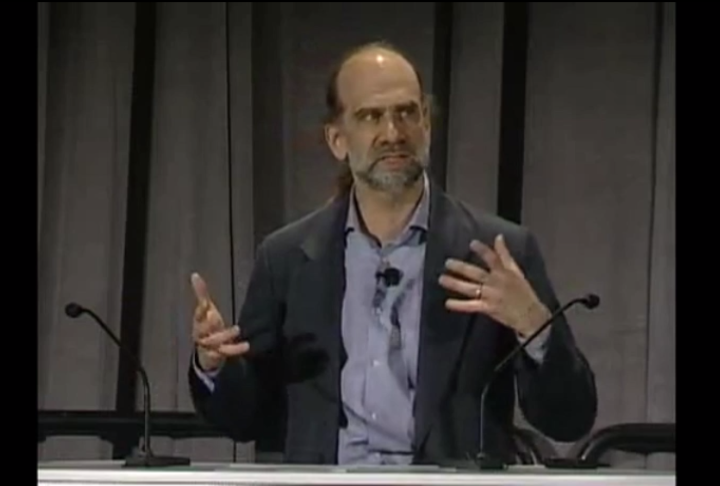
\includegraphics[width = \textwidth]{figures/schneider.png}}{figures/SchneiderTalk.mp4}

\end{frame}

\note{This economic relation was first termed as ``product is you'' by Security Researcher Bruce Schneider at Harvard. He does a much better job of summing it up than I could. This is him talking at RSA conference in 2010.}

\begin{frame}
	\frametitle{Who is Tracking You?}

	Other people	\vspace{1em}    

	\textbf{Businesses} \vspace{1em}

	Governments	\vspace{1em}

\end{frame}

\note{We talk about other people tracking you online in Cyberbullying module.

Our focus on this module is the businesses that are tracking you.}

\begin{frame}
	\frametitle{What Do They Know?}

	    \begin{columns}
			\begin{column}{0.5\textwidth}
			
			What you give them:

			\begin{itemize}
				\item Your posts
				\item Your pictures
				\item Account information
				\item Payment information
			\end{itemize}	
	
			\end{column}

			\begin{column}{0.5\textwidth}
	
			\only<2>{
			What you generate:

			\begin{itemize}
				\item Cookies
				\item Network Addresses
				\item Hardware Identifiers
				\item Location Data
				\item Biometric Markers
				\item Browser Fingerprints
			\end{itemize}
			}
	
			\end{column}
	
		\end{columns}

\end{frame}

\note{One might think a forum knowing what your alias posted on there is no big deal. What can they do knowing CuteCat99 posts cat pictures on r/aww?

You may feel in control of the information you share with the forum. Thinking it is all they have on you.

The companies don't just rely on what you give them. They also obtain the digital footprints you leave behind as you browse.

They don't only rely on data they themselves can obtain, they also correlate this data across the internet.}

\begin{frame}
	\frametitle{Hey! I like cookies!}
    
        \begin{columns}
    		\begin{column}{0.5\textwidth}
    
    			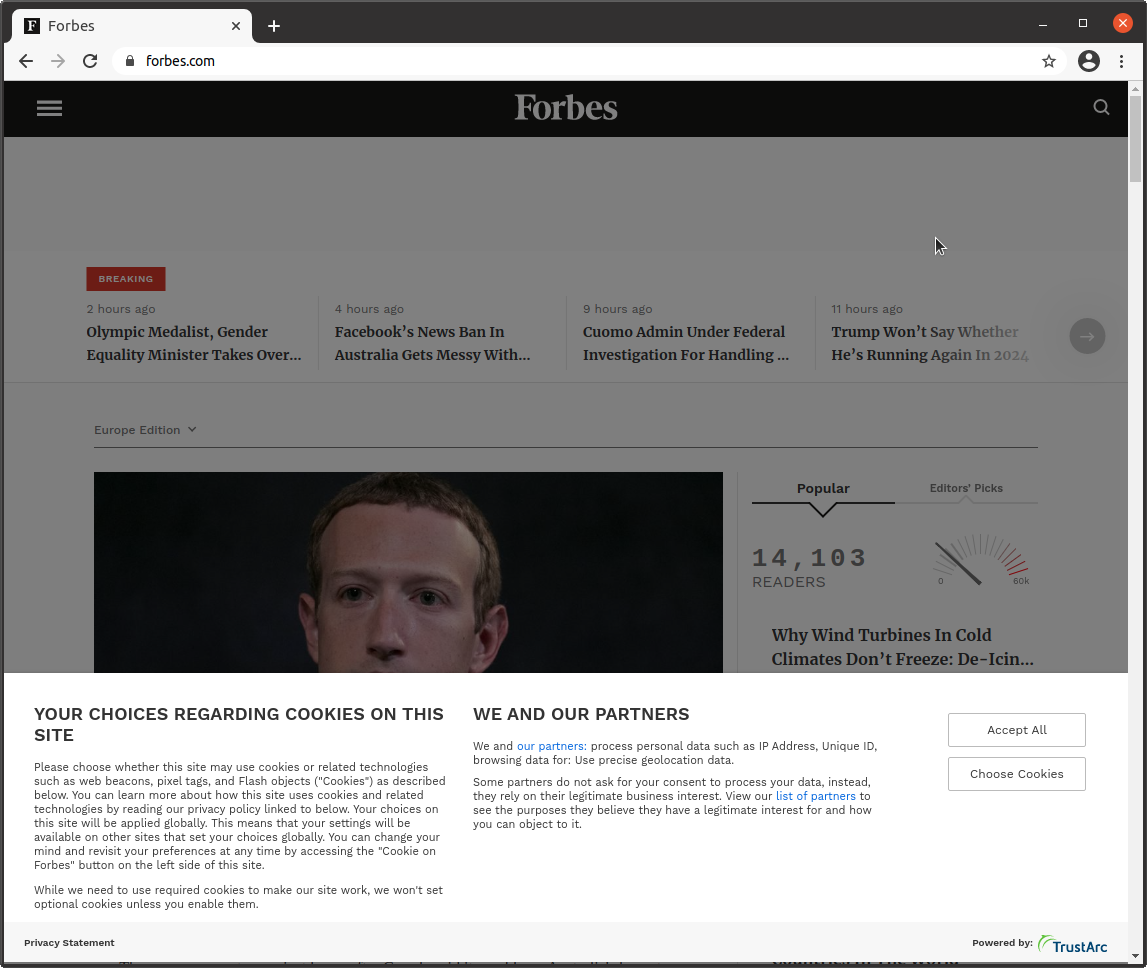
\includegraphics[width = \textwidth, height = .85\textheight, keepaspectratio]{figures/cookies2.png}
    	
    		\end{column}
    
    		\begin{column}{0.5\textwidth}
    
    			
\includegraphics[width = \textwidth, height = .85\textheight, keepaspectratio]{figures/bd1.jpg}
    
    		\end{column}
    
    	\end{columns}

\end{frame}

\note{Cookies are small files stored on your computer. Each time you visit a web site the cookie for that site gets shared with them. That is why you don't have to login every time you visit the site.

There is a more sinister use for these cookies. By tracking cookies across the sites, advertisers can track your activities across multiple web sites.}

\begin{frame}
	\frametitle{How Much Can They Know?}
    
	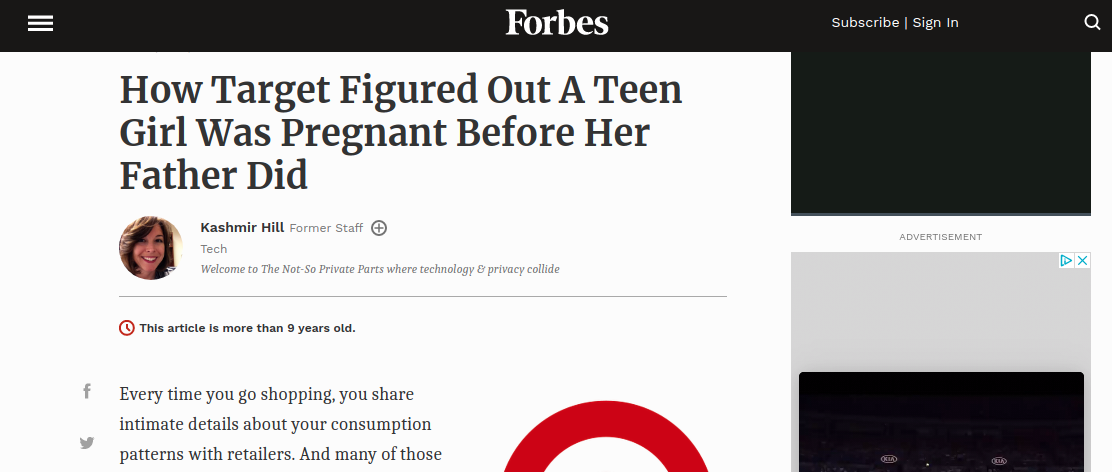
\includegraphics[width = \textwidth, height = .85\textheight, keepaspectratio]{figures/target.png}

\end{frame}

\note{There is the famous Target story from a few years back.

How do they know so much?

They correlate the identifiers across the internet to build behavioral profiles. So they don't only know you posted cat pictures as CuteCat99 on r/aww, but the same cell phone also visited Wineshops in Valby. The same cell phone had stored touchless payment card information, which was used to buy cat food, wine, and the book ``subtle art of not giving a fuck''. The payment card information had the name of the person, so now google knows who CuteCat99 is and classifies her as a cat lady.}

\begin{frame}
	\frametitle{How Do They Monetize This?}
    
    \centering

	\includegraphics<1>[width = \textwidth, height = .85\textheight, keepaspectratio]{figures/bid1.png}

	\includegraphics<2>[width = \textwidth, height = .85\textheight, keepaspectratio]{figures/bid2.png}

	\vfill \tiny{Source: Behind the One-Way Mirror, EFF, 2018}

\end{frame}

\note{In the time it takes to load the website, the advertisers conduct and auction for the placement of an ad on your browser window. Sell the spot to the highest bidder and place tha ad on the web site.

The add network receives the request for an add from your web browser. Based on the information the network has on you it creates a bid request. The advertisers look at the personal information and make a bid to show advertisement. Add network goes through matching bids such as young female interested in first person shooters and pick the highest bid to serve the add to you. Then you get served the add for Call of Duty MXVII.

The advertisers place bids for their targeted customers: An insurance company may be interested in people looking to buy cars, a make up company may be interested in women with a high purchasing power, a gym may be interested in young professionals in a certain neighborhood for example.}

\begin{frame}
	\frametitle{Defence Against Dark Arts}
    
	    \begin{columns}
			\begin{column}{0.5\textwidth}
			
			    GDPR is your friend! \vspace{1em}

			    Consider GDPR warnings \vspace{1em}

			    Use tracker blockers \vspace{1em}

			    Consider app permissions \vspace{1em}

			    Don't engage with services you don't need
		
			\end{column}
	
			\begin{column}{0.5\textwidth}
	
				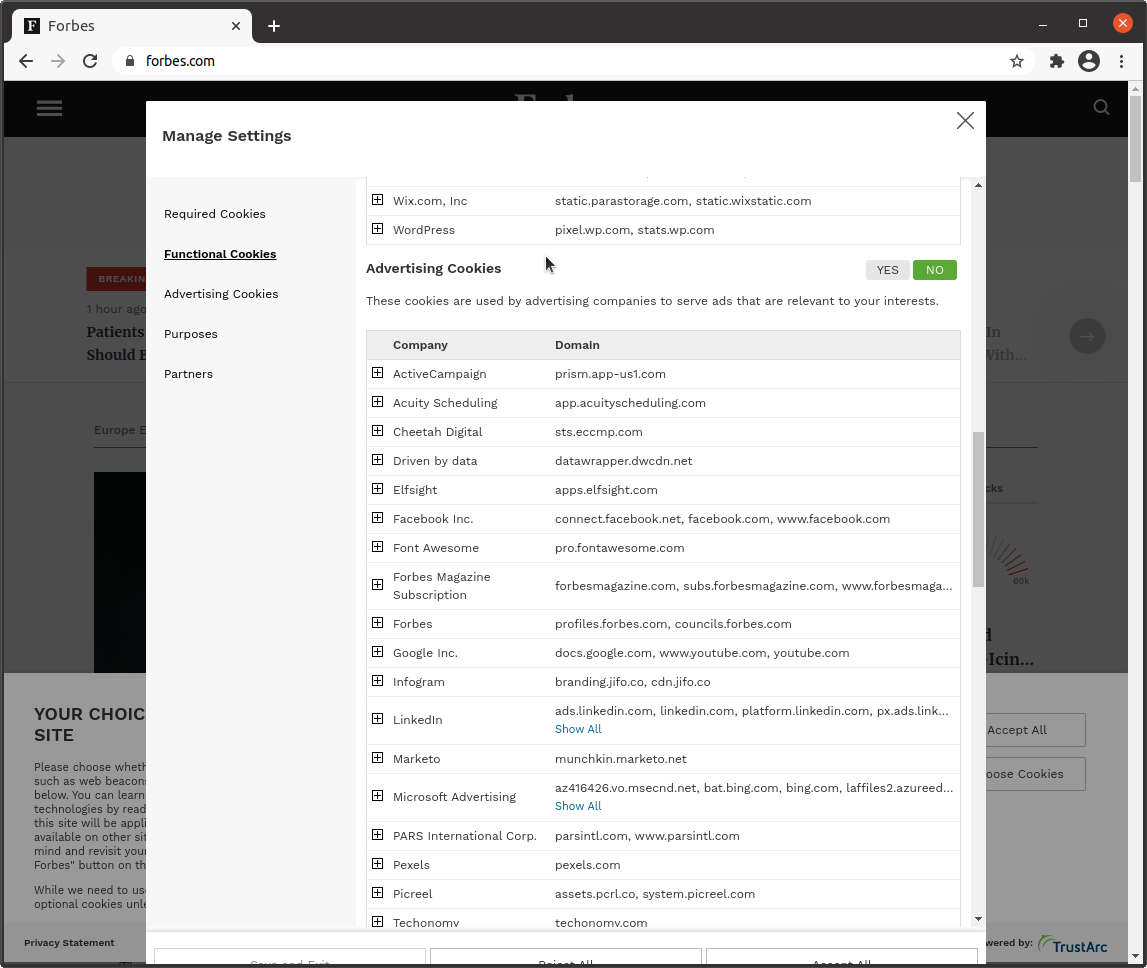
\includegraphics[width = \textwidth, height = .85\textheight, keepaspectratio]{figures/cookies3.png}
	
			\end{column}
	
		\end{columns}

\end{frame}

\end{document}
